\documentclass[12pt,a4paper,openany,twoside,cap]{ctexbook}
%-------------------------------------宏包引用---------------------------------------------------
\usepackage[paperwidth=216mm,paperheight=279mm,textwidth=176mm,textheight=239mm,left=20mm,right=20mm, top=25mm, bottom=20mm]{geometry}            %定义版面: letter
%--------------------------------------------------------------------------------------
\usepackage{fontspec}
\usepackage{xunicode}
\usepackage{xltxtra}
\usepackage{everb}
\usepackage{listings}
\usepackage{mdwlist}
\usepackage{longtable}
\usepackage{amsfonts,amssymb}
%--------------------------------------------------------------------------------------
\usepackage[skins,listings,breakable,theorems]{tcolorbox}

\usepackage{fancybox}                 % 边框,有阴影,fancybox提供了五种式样\fbox,\shadowbox,\doublebox,\ovalbox,\Ovalbox。
\usepackage{colortbl}                 % 单元格加背景
\usepackage{fancyhdr}                 % 页眉和页脚的相关定义
\usepackage[unicode, colorlinks, bookmarksnumbered=true,pdfstartview=FitH,linkcolor=blue,citecolor=red,urlcolor=magenta]{hyperref}   % 书签功能,选项去掉链接红色方框

%\setmonofont{Consolas}               % Consolas字体,字母符号连用有问题

\usepackage{chngcntr}                 % 公式、图的编号不显示章节号
\counterwithout{equation}{chapter}
\counterwithout{equation}{section}
\counterwithout{figure}{chapter}
\counterwithout{figure}{section}

\usepackage{bigfoot}                  % use \verb in footnote

\usepackage{listings,xcolor}
\lstset{
        extendedchars=false,          % non-English characters
        lineskip=2pt,
%%        backgroundcolor=\color{white},
        basicstyle=\tt\footnotesize\color{black},   % 字体大小和颜色
        commentstyle=\tt\color{green!40!black},
        keywordstyle=\tt\color{blue},
        stringstyle=\tt\color{magenta},
        showspaces=false,             % underline spaces in the codes
        showstringspaces=false,       % underline spaces only in a string
        showtabs=false,               % underline tabs in the codes
%%        identifierstyle=\tt\color{red!60!black},
        numbers=left,
        numberstyle=\tiny\color{black},
        numberstyle=\scriptsize\color{red!75!black},
        numbersep=14pt,               % how far the line-numbers are from the code
        texcl=false,                  % comments in LaTeX if true
%        emph={                        % keywords to be highlighted
%               subroutine, return,
%               end
%        },
        emphstyle=\sf\bfseries\color{red!50!black}\fcolorbox{orange!40!white}{.},
%%        rulecolor=\color{green},
%%        frame=single,
%%        frame=shadowbox,
        tabsize=2,                    % set default tab-size to 2 spaces
}

\newtcblisting{commandshell}{colback=black,colupper=white,colframe=yellow!75!black,
%listing only,listing options={style=tcblatex,language=sh,numbers=none},
listing only,listing options={style=tcblatex,numbers=none},
every listing line={\textcolor{red}{\small\ttfamily\bfseries UserID \$> }}}

%\newtcblisting{molprojob}{
%breakable,colback=green!5!white,colframe=green!75!black,left=7mm,
%enhanced,
%listing only,
%listing options={aboveskip=0pt,belowskip=0pt,basicstyle=\ttfamily,numbers=left,
%    numberstyle=\scriptsize\color{red!75!black}},
%overlay={\begin{tcbclipinterior}\fill[red!20!blue!20!white] (frame.south west)
%    rectangle ([xshift=5mm]frame.north west);\end{tcbclipinterior}}
%}
   %引用宏包所在位置
%-----------------------------------------------------主文档 格式定义---------------------------------
\addtolength{\headsep}{-0.1cm}        %页眉位置
%\addtolength{\footskip}{0.4cm}       %页脚位置
%-----------------------------------------------------设定字体等------------------------------
\setmainfont{Times New Roman}    % 缺省字体
\setCJKfamilyfont{song}{SimSun}
\setCJKfamilyfont{hei}{SimHei}
\setCJKfamilyfont{kai}{KaiTi}
\setCJKfamilyfont{fs}{FangSong}
\setCJKfamilyfont{li}{LiSu}
\setCJKfamilyfont{you}{YouYuan}
\setCJKfamilyfont{yahei}{Microsoft YaHei}
\setCJKfamilyfont{xingkai}{STXingkai}
\setCJKfamilyfont{xinwei}{STXinwei}
\setCJKfamilyfont{fzyao}{FZYaoTi}
\setCJKfamilyfont{fzshu}{FZShuTi}
%-------------------------------------------------------------------
%  CTex/XeLaTeX和(Windows) TexLive/XeLaTeX通用
\newcommand{\song}{\CJKfamily{song}}           % 宋体   (Windows自带simsun.ttf)
\newcommand{\fs}{\CJKfamily{fs}}               % 仿宋体 (Windows自带simfs.ttf)
\newcommand{\kai}{\CJKfamily{kai}}             % 楷体   (Windows自带simkai.ttf)
\newcommand{\hei}{\CJKfamily{hei}}             % 黑体   (Windows自带simhei.ttf)
\newcommand{\li}{\CJKfamily{li}}               % 隶书   (Windows自带simli.ttf)
%  或者,仅TexLive/XeLaTeX,支持更多字体
%\newCJKfontfamily\song{SimSun}
%\newCJKfontfamily\hei{SimHei}
%\newCJKfontfamily\kai{KaiTi}
%\newCJKfontfamily\fs{FangSong}
%\newCJKfontfamily\li{LiSu}
%\newCJKfontfamily\you{YouYuan}
%\newCJKfontfamily\yahei{Microsoft YaHei}
%\newCJKfontfamily\xingkai{STXingkai}
%\newCJKfontfamily\xinwei{STXinwei}
%\newCJKfontfamily\fzyao{FZYaoTi}
%\newCJKfontfamily\fzshu{FZShuTi}
%------------------------------------------------------------定义颜色--------------
\definecolor{blueblack}{cmyk}{0,0,0,0.35}%浅黑
\definecolor{darkblue}{cmyk}{1,0,0,0}%纯蓝
\definecolor{lightblue}{cmyk}{0.15,0,0,0}%浅蓝
%--------------------------------------------------------设定标题颜色------------------
\CTEXsetup[format+={\color{darkblue}}]{chapter}
\CTEXsetup[format+={\color{darkblue}}]{section}
\CTEXsetup[format+={\color{darkblue}}]{subsection}
%--------------------------------------------------------表格边框颜色------------------
\arrayrulecolor{darkblue}
%------------------------------------------------------定义、定理环境------------------
\newcounter{myDefinition}[chapter]\def\themyDefinition{\thechapter.\arabic{myDefinition}}
\newcounter{myTheorem}[chapter]\def\themyTheorem{\thechapter.\arabic{myTheorem}}
\newcounter{myCorollary}[chapter]\def\themyCorollary{\thechapter.\arabic{myCorollary}}

\tcbmaketheorem{defi}{定义}{fonttitle=\bfseries\upshape, fontupper=\slshape, arc=0mm, colback=lightblue,colframe=darkblue}{myDefinition}{Definition}
\tcbmaketheorem{theo}{定理}{fonttitle=\bfseries\upshape, fontupper=\slshape, arc=0mm, colback=lightblue,colframe=darkblue}{myTheorem}{Theorem}
\tcbmaketheorem{coro}{推论}{fonttitle=\bfseries\upshape, fontupper=\slshape, arc=0mm, colback=lightblue,colframe=darkblue}{myCorollary}{Corollary}
%--------------------------------------------------------------------------------------
\newtheorem{proof}{\indent\hei \textcolor{darkblue}{证明}}
\newtheorem{Solution}{\indent\hei \textcolor{darkblue}{解}}
%----------------------------------------------------定义页眉下单隔线-------------------
\newcommand{\makeheadrule}{\makebox[0pt][l]{\color{darkblue}\rule[.7\baselineskip]{\headwidth}{0.3pt}}\vskip-.8\baselineskip}
%-----------------------------------------------定义页眉下双隔线----------------
\makeatletter
\renewcommand{\headrule}{{\if@fancyplain\let\headrulewidth\plainheadrulewidth\fi\makeheadrule}}
\pagestyle{fancy}
\fancyhf{} %清空页眉
\fancyhead[RO]{\kai{\footnotesize.~\color{darkblue}\thepage~.}}         % 奇数页码显示左边
\fancyhead[LE]{\kai{\footnotesize.~\color{darkblue}\thepage~.}}         % 偶数页码显示右边
\fancyhead[CO]{\song\footnotesize\color{darkblue}\rightmark} % 奇数页码中间显示节标题
\fancyhead[CE]{\song\footnotesize\color{darkblue}\leftmark}  % 偶数页码中间显示章标题
%---------------------------------------------------------------------------------------------------------------------
    %格式所在位置
\begin{document}
\pagenumbering{Roman}       %Roman字体书写页码

%---------------------------------------------------封面--------------------------
\title{
\vspace{-3cm}
\zihao{1}\hei\textsc{UniMoVib}使用手册  \\
\vspace{1cm} \zihao{3}(1.2.1版)\vspace{30 mm} \\
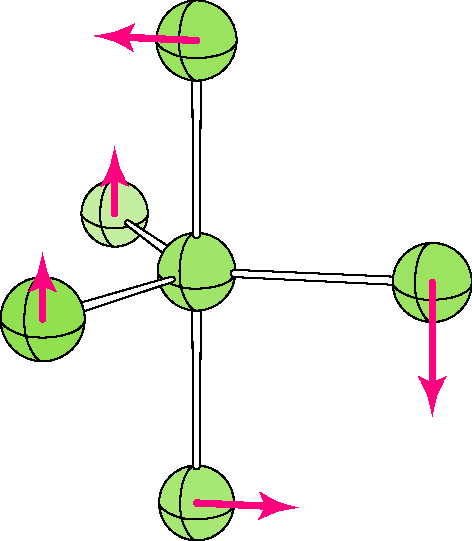
\includegraphics[width=50.0mm]{fig/logo} \vspace{30 mm}}

\author{
\textbf{邹文利} \\ \vspace{5mm}
西北大学现代物理研究所,西安,710127 \\ \vspace{5mm}
\href{mailto:qcband@gmail.com}{qcband@gmail.com}
}

\date{\vspace{1cm}  \today}
\maketitle

%-------------------------------------目录----------------------------------------
\setcounter{page}{1}   %重新开始页码
\renewcommand\contentsname{目\qquad 录}
% 下面三行去掉了目录首页页码
\makeatletter
\let\ps@plain\ps@empty
\makeatother
\tableofcontents            %目录

%-----------------------------------------正文开始----------------------------------
\mainmatter
\chapter{关于\textsc{UniMoVib}}
\label{part:about}

\textsc{UniMoVib}是进行分子振动频率计算的统一接口。程序最初是我于2014至2015年在德州达拉斯市的南方卫理会大学期间用 FORTRAN 77编写,用作\href{https://sites.smu.edu/dedman/catco/}{CATCO小组}的分子局域模式程序\href{https://github.com/catco-smu}{\textsc{LocalMode}}的前端接口。本项工作得到美国NSF项目CHE 1152357和CHE 1464906的支持,并得到已故 的Dieter Cremer教授的鼎力支持和指导。
从2017年春天开始,\textsc{UniMoVib}用Fortran 90重新改写,作为独立程序发布。

\section{功能} \label{sec:feature}

\begin{itemize}
\item 从 Hessian、坐标等数据计算谐振频率和(可选的)红外强度,这些数据可以由量子化学程序产生,或者由用户手工编写。 \\
目前已经支持近30个量子化学程序(参见第\ref{sec:inp-contrl}节),尽管有些程序可能自己做得更好。
\item 分析结构的最高点群以及简正振动模式的不可约表示(\emph{irreps.})。(\emph{irreps.}:仅闭壳层分子。) \\
对称性分析基于\textsc{Mopac} 7.1程序包中的对称性子程序,\textsc{Mopac} 7.1的源代码已经开放,不受版权限制(参见\href{http://openmopac.net/Downloads/Downloads.html}{openmopac.net} and \href{https://sourceforge.net/projects/mopac7/}{sourceforge.net})。
\item 使用最高点群做热化学计算,并打印 Gaussian风格的热化学计算结果(详细解释,参见: Foresman and Frisch, \emph{Exploring Chemistry With Electronic Structure Methods}, Ed.2, Gaussian Inc., Pittsburgh, PA, \textbf{1996}, pp.66)。
\item 保存\textsc{Molden}文件,用于动画显示振动模式。
\item 设定同位素,温度,压强,频率换算因子或实验频率,等。
\item 可作为量子化学程序(尤其是不支持非阿贝尔点群的程序)的第三方模块,用于频率和热化学计算。
\end{itemize}

\section{对称性} \label{sec:symm}

程序支持的点群列于表\ref{tab:symm}中。

程序会打印分子的两个点群对称性,即``\verb|Electronic Wavefunctions|''的点群对称性和 \\
``\verb|Nuclear & Total Wavefunctions|''的点群对称性。二者的区别是,前者不依赖同位素质量,而后者依赖同位素质量。应当用后者去分析振动模式和进行热化学计算。不过,有些量子化学程序并不是这么做的,导致无法分析振动模式的不可约表示,并导致错误的Gibbs自由能。
一个极端的例子是富勒烯$^{12}$C$_{59}{}^{13}$C,其电子波函的对称性是$I_h$,而核波函以及总波函的对称性是$C_1$。若热化学计算使用$I_h$,Gibbs自由能的误差将会达到 2.5 kcal/mol!

\begin{table}[!htbp]
\caption{可用的点群}\label{tab:symm}
\small\centering
\begin{tabular}{ll}
\hline\hline
$C_{n}$           & n = 1\ldots 8 \\
$C_s$, $C_{nv}$   & n = 2\ldots 8 \\
$C_i$, $C_{nh}$   & n = 2\ldots 8 \\
$D_{n}$           & n = 2\ldots 8 \\
$D_{nd}$          & n = 2\ldots 7 \\
$D_{nh}$          & n = 2\ldots 8 \\
$S_{n}$           & n = 4, 6, 8 \\
其它            & $R_3$, $T$, $T_d$, $T_h$, $O$, $O_h$, $I$, $I_h$, $C_{\infty v}$, $D_{\infty h}$ \\
\hline\hline
\end{tabular}
\end{table}


\chapter{编译与运行} \label{part:setting}

\section{编译程序} \label{sec:install}

\begin{commandshell}
cd $UniMoVib/src
make
\end{commandshell}
需要在\verb|Makefile|中定义合适的Fortran90编译器。


\section{运行程序} \label{sec:run}

运行方法:\\
用鼠标双击二进制程序\verb|unimovib.exe|,并键入输入文件名(仅MS-Windows),

或者 \\
在终端中键入
\begin{commandshell}
./unimovib.exe
\end{commandshell}
\noindent 接下来,键入输入文件名(若不提供输入文件名,使用默认文件名\verb|job.inp|),

或者 \\
在终端中键入
\begin{commandshell}
./unimovib.exe -b < input > output
\end{commandshell}

最后一种方式可以用来准备批处理脚本,做一系列计算。


\chapter{输入说明} \label{part:input}

输入选项按照namelist分组,每一组结束用\verb|$END|。这些组的输入顺序任意。注意:每个\verb|$|符号之前,至少要有一个空格。

输入内容不区分大小写,但\verb|$QCData|输入组中的数据文件名除外(参见第\ref{sec:inp-qcdata}节)。

\section{\texttt{\$Contrl}输入组} \label{sec:inp-contrl}

该输入组指定计算类型。关键词:

\bigskip{}
\verb|QCProg="XXXX"|: \verb|XXXX|是计算分子 Hessian和振动频率的量子化学程序名。支持以下程序:
\begin{itemize}
\item \verb|Gaussian| (默认)。
\item \verb|GAMESS| (同义词:\verb|GAMESS-US|,\verb|GAMESSUS|)。
\item \verb|Firefly| (同义词:\verb|PCGamess|,\verb|PC-Gamess|)。
\item \verb|GAMESS-UK| (同义词:\verb|GAMESSUK|)。
\item \verb|ORCA|。
\item \verb|Molpro|。
\item \verb|QChem| (同义词:\verb|Q-Chem|)。
\item \verb|NWChem|。
\item \verb|CFour|。
\item \verb|Turbomole|。
\item \verb|deMon2k| (同义词:\verb|deMon|)。
\item \verb|PQS|。
\item \verb|OpenMOPAC| (同义词:\verb|MOPAC|)。同时支持\textsc{Mopac} 6和\textsc{Mopac} 7,但\textsc{Fujitsu Mopac} 200x(如今是\textsc{Scigress}中的MO-G模块)未测试。
\item \verb|AMSOL| (同义词:\verb|AMPAC|)。支持\textsc{Ampac} 2.x,但以后版本的\textsc{Ampac}未测试。
\item \verb|Dalton|。
\item \verb|FHI-AIMS| (同义词:\verb|FHIAIMS|,\verb|AIMS|)。
\item \verb|CP2k|。\textsc{QuickStep}模块。
\item \verb|Hyperchem|。
\item \verb|Jaguar|。\textsc{Schr\"odinger Suite}中的量子化学计算模块。
\item \verb|ADF|。仅支持分子模块\textsc{Adf}。
\item \verb|MOLDEN|。由频率计算产生,至少应当包含以下三部分:\verb|[FREQ]|,\verb|[FR-COORD]|,\verb|[FR-NORM-COORD]|。 \textsc{Aces-II},\textsc{Columbus},\textsc{Dalton} (解析频率计算),\textsc{Molcas}等程序都可以通过\textsc{Molden}文件被支持。
\item \verb|Crystal|。支持分子谐振频率计算,只对\textsc{Crystal} 14进行了测试。
\item \verb|Spartan|。
\item \verb|PSI|。仅对\textsc{Psi} 4进行了测试。
\item \verb|DMOL3| (同义词:\verb|DMOL|)。仅支持分子的谐振频率计算。
\item \verb|ACES|。对\textsc{Aces-II}和\textsc{Aces-III}都进行了测试。
\item \verb|UniMoVib| (同义词:\verb|ALM|)。\textsc{UniMoVib}产生的纯文本数据文件。参见附录\ref{sec:almfmt}。
\end{itemize}
\verb|     |此外,\verb|QCProg="AtomCalc"|可用于做原子热化学计算(参见第\ref{sec:inp-atom}节)。

\bigskip{}
\verb|Isotop|:设定同位素质量。
\begin{description}
\item[ ]\verb|  = 0|:(默认)从频率计算的数据文件读入全部原子量;若不存在,原子量从程序的数据库读取(除个别程序外,都使用最丰同位素质量)。
\item[ ]\verb|  = 1|:从频率计算的数据文件或程序的数据库读入全部原子量(同\verb|0|),但是接下来,指定原子序号的同位素质量将用\verb|$IsoMas|输入组(参见第\ref{sec:inp-isomas}节)后的质量替换。
\item[ ]\verb|  = 2|:所有的原子质量都在\verb|$IsoMas|输入组(参见第\ref{sec:inp-isomas}节)之后提供。
\end{description}

\bigskip{}
\verb|IFExp|:(\verb|.True.|/\verb|.False.|)用实验振动频率校正Hessian矩阵,在\verb|$ExpFrq|输入组(参见第\ref{sec:inp-expfrq}节)之后提供。默认:\verb|.False.|

\bigskip{}
\verb|IFSAVE|:(\verb|.True.|/\verb|.False.|)把原子质量(受\verb|Isotop|影响),直角坐标,Hessian矩阵(受\verb|IFExp|影响),APT矩阵保存到纯文本数据文件*.umv中。该关键词不能与\verb|QCProg="AtomCalc"|或\verb|"UniMoVib"|同时用。默认:\verb|.False.|。关于数据格式,参见附录\ref{sec:almfmt}。

\bigskip{}
\verb|IFMOLDEN|:(\verb|.True.|/\verb|.False.|)除了\verb|QCProg="AtomCalc"|或\verb|"MOLDEN"|之外,保存\textsc{Molden}文件,它可以用\href{http://www.cmbi.ru.nl/molden/molden.html}{\textsc{Molden}}或\href{http://gabedit.sourceforge.net/}{\textsc{Gabedit}}程序打开,用于显示分子结构和振动模式。默认:\verb|.False.|

\bigskip{}
\verb|IFLOCAL|:(\verb|.True.|/\verb|.False.|)保存数据文件,用于\textsc{LocalModes}程序的局域模式分析(主页:\href{https://github.com/catco-smu}{https://github.com/catco-smu})。该关键词不能用于
\verb|QCProg="AtomCalc"|。默认:\verb|.False.|。

\bigskip{}
\verb|IFGauTS|:(\verb|.True.|/\verb|.False.|)把结构和Hessian矩阵存为\textsc{Gaussian}的输入文件模板,用于过渡态优化计算。该关键词不能用于
\verb|QCProg="AtomCalc"|。默认:\verb|.False.|。注意:此输入对于ONIOM计算类型无效,因为\textsc{Gaussian}此时只能使用默认的冗余内坐标进行优化。

\subsection{专家级关键词} \label{subsec:inp-qcdata-expert}

一般不需要在\texttt{\$Contrl}中设置这些关键词。

\bigskip{}
\verb|QCProg="XYZ"|:仅用于调试。

\bigskip{}
\verb|IFConc|:(\verb|.True.|/\verb|.False.|)控制是否简明频率输出。默认:\verb|.False.|

\bigskip{}
\verb|ISyTol = MN|:判断对称性的精度阈值$M*10^{N-3}$,其中M总为正数,正负号只分配给N。于是,\verb|ISyTol = 21|表示0.02,而\verb|-21|表示0.0002。默认:10,即0.001。

\bigskip{}
\verb|IFRdNM|:(\verb|.True.|/\verb|.False.|)是否从\texttt{\$QCData}输入组指定的数据文件直接读取简正模式,避免做对角化,从而节省内存并加快计算速度。若设定该关键词,不能同时用\verb|Isotop|设定同位素质量,或者用\verb|IFExp=.True.|进行振动频率校正。该关键词目前仅支持\verb|QCProg="Gaussian"|。默认:\verb|.False.|。

\bigskip{}
\verb|IFApprx|:(\verb|.True.|/\verb|.False.|)是否从外部文件读取内坐标力常数(伸缩:mDyn/\AA,角度:mDyn$\cdot$\AA/Rad$^2$)和Wilson B矩阵,并构造近似的Hessian矩阵进行简正振动频率计算。数据文件在\texttt{\$QCData}输入组指定。该关键词不能与\verb|IFRdNM=.True.|同时使用。默认:\verb|.False.|。

%\newpage

\section{\texttt{\$QCData}输入组} \label{sec:inp-qcdata}

这一输入组指定数据文件(包含原子质量,坐标,APT,和 Hessian),用双引号括起。一般只需要一个数据文件,由选项\verb|FCHK|指定,但是对于有些程序,需要使用关键词
\verb|HESS|,\verb|DDIP|,和/或\verb|GEOM|指定多个数据文件。

若\verb|IFApprx=.True.|,构造近似Hessian矩阵的数据文件由\verb|BMAT|指定。

\begin{itemize}
\item \textsc{Gaussian}:*.fchk。默认情况下,fchk文件 不包含原子质量,于是程序假定为最丰同位素质量。但是对于\textsc{Gaussian} 09(以及更高的版本),可以用\texttt{FREQ(SaveNormalModes)}把原子质量保存到fchk文件。用关键词\texttt{FREQ(Raman)}可以保存拉曼强度计算所需的极化率导数。
\item \textsc{Gamess}:*.dat(通过\verb|FCHK|) + *.out(通过\verb|GEOM|)。
\item \textsc{Firefly}:data文件(通过\verb|FCHK|;默认为\verb|PUNCH|) + *.out(通过\verb|GEOM|)。
\item \textsc{Gamess-uk}:*.out文件。如果对红外强度感兴趣,可以在频率计算中指定关键词\texttt{RUNTYPE INFRARED},用于输出APT。
\item \textsc{Orca}:*.hess。
\item \textsc{Molpro}:*.out文件。用以下命令打印Hessian和APT: \\
\verb|{frequencies,print=1;print,hessian}|
\item \textsc{Q-Chem}:*.fchk。在\textsc{Q-Chem}的频率计算中,用\texttt{GUI=2}产生*.fchk文件。fchk文件不包含原子质量,程序假定为最丰同位素质量。
\item \textsc{NWChem}:*.out文件(通过\verb|FCHK|) + *.fd{\_}ddipole (通过\verb|DDIP|) +
*.hess (通过\verb|HESS|),其中\verb|DDIP|是可选的,若对红外强度不感兴趣可以忽略。
\item \textsc{CFour}
  \begin{description}
  \item[ ]解析频率计算(\texttt{VIB=ANALYTIC}):*.out文件(通过\verb|FCHK|) + GRD(通过\verb|GEOM|)。
  \item[ ]数值频率和解析频率计算:使用\textsc{Molden}文件。但是无红外强度。参见下面的\texttt{MOLDEN}。
  \end{description}
\item \textsc{Turbomole}:aoforce模块的*.out文件(通过\verb|FCHK|;默认:aoforce.out) +
dipgrad(通过\verb|DDIP|),其中\verb|DDIP|是可选的,若对红外强度不感兴趣可以忽略。
\item \textsc{deMon2k}:*.out文件(通过\verb|FCHK|;默认:deMon.out)。\textsc{deMon2k}可以通过\texttt{PRINT DE2}打印Hessian。
\item \textsc{Pqs}:*.coord文件(通过\verb|FCHK|) + *.deriv(通过\verb|DDIP|) + *.hess(通过\verb|HESS|),其中\verb|DDIP|是可选的,若对红外强度不感兴趣可以忽略。
\item \textsc{OpenMopac}:*.out文件(通过\verb|FCHK|)。使用\texttt{FORCE DFORCE}或
\texttt{FORCE=DFORCE}打印Hessian。使用平均原子量,可能与非常早期版本的\textsc{Mopac}不一致。
\item \textsc{Amsol}:*.out文件(通过\verb|FCHK|)。使用\texttt{FORCE DFORCE}打印Hessian。使用平均原子量,可能与非常早期版本的\textsc{Amsol/Ampac}不一致。
\item \textsc{Dalton}:*.out文件(通过\verb|FCHK|)。由于\textsc{Dalton}不打印核电荷数和元素符号,因此在\textsc{Dalton}频率计算的输入文件中,必须指定标准的元素符号(例如,Mg可以,而Mg01、Mgxx则不行)。
\item \textsc{Fhi-Aims}:masses.*.dat文件(通过\verb|FCHK|) + grad{\_}dipole.*.dat(通过\verb|DDIP|) + hessian.*.dat(通过\verb|HESS|),其中\verb|DDIP|是可选的,若对红外强度不感兴趣可以忽略。
\item \textsc{CP2k}:\textsc{Quickstep}模块频率计算产生的输出文件(通过\verb|FCHK|)。
\item \textsc{HyperChem}:频率计算的日志文件(通过\verb|FCHK|)。
\textsc{HyperChem}默认不产生日志文件。在做频率计算前,来到\textbf{File}菜单,选择\textbf{Save log}的打印级别为9,就可以保存日志文件。
\item \textsc{Jaguar}:频率计算的输出文件(通过\verb|FCHK|)。
\item \textsc{Adf}:格式化的数据文件TAPE21或TAPE13(通过\verb|FCHK|)。数值频率计算时有些问题,参见第\ref{part:problem}章。
\item \textsc{Molden}:数据文件(通过\verb|FCHK|),其中包含\verb|[FREQ]|,
\verb|[FR-COORD]|,\verb|[FR-NORM-COORD]|数据区。一些问题参见第\ref{part:problem}章。
\item \textsc{Crystal}:分子谐振频率计算产生的输出文件(通过\verb|FCHK|)。
\item \textsc{Spartan}:*.smol存档文件(通过\verb|FCHK|)。假定为最丰同位素质量。
\item \textsc{Psi}:输出文件(通过\verb|FCHK|)。在\textsc{Psi} 4的频率计算中,用\texttt{set print 3}打印Hessian。
\item \textsc{Dmol3}:输出文件(通过\verb|FCHK|)。
\item \textsc{Aces}:输出文件(通过\verb|FCHK|),但是建议使用\textsc{Molden}文件,可以得到更高的数字精度。 一些问题参见第\ref{part:problem}章。
\item \textsc{UniMoVib}:ASCII数据文件(通过\verb|FCHK|),\textsc{UniMoVib}通过选项\verb|IFSAVE=.TRUE.|产生,也可以由用户手工编写(参见附录\ref{sec:almfmt})。
\item XYZ:标准的XYZ数据文件(通过\verb|FCHK|)。仅用于调试。
\end{itemize}

参见\verb|$UniMoVib/test|中的示例。

\section{\texttt{\$IsoMas}输入组} \label{sec:inp-isomas}

\verb|Isotop = 1|或\verb|2|时需要该输入组。输入组不需要选项。输入组之后,提供同位素质量。

\bigskip{}
若\verb|Isotop = 1|,每行定义一个原子,包括原子序号及质量。程序连续读取,直到遇到空行或输入结束为止。例如,
\begin{colorboxed}[oval=false,boxcolor=green!75!black,bgcolor=green!5!white]
\ttfamily
\begin{lstlisting}
 $IsoMas $End
2 15.99491
4  2.01410
\end{lstlisting}\end{colorboxed}
这里指定第二和第五个原子的质量分别为15.99491和2.01410。

\bigskip{}
若\verb|Isotop = 2|,全部N个原子的质量以自由格式提供。例如,
\begin{colorboxed}[oval=false,boxcolor=green!75!black,bgcolor=green!5!white]
\ttfamily
\begin{lstlisting}
 $IsoMas $End
12.0 1.0 1.0
1.0
1.0
\end{lstlisting}\end{colorboxed}
以上定义了 CH$_4$的5个原子质量。

\section{\texttt{\$ExpFrq}输入组} \label{sec:inp-expfrq}

\verb|IFExp=.True.|时需要该输入组。该输入组只有一个选项\verb|MODE|。在该选项组之后,提供频率实验值。

\bigskip{}
若\verb|MODE = 0|(默认),以自由格式定义所有的$N_{Vib}$个振动频率值,它们必须正确地排序,与频率计算值一致。例如:
\begin{colorboxed}[oval=false,boxcolor=green!75!black,bgcolor=green!5!white]
\ttfamily
\begin{lstlisting}
 $ExpFrq $End
 835.0248 835.3904 926.0930 926.2148
 2160.9759
\end{lstlisting}\end{colorboxed}


若\verb|MODE = 1|,一系列理论频率值将用实验频率值替代。每行一个频率,包括频率的编号,及其实验值。程序连续读取,直到遇到空行或输入结束为止。例如,
\begin{colorboxed}[oval=false,boxcolor=green!75!black,bgcolor=green!5!white]
\ttfamily
\begin{lstlisting}
 $ExpFrq MODE=1 $End
 3  926.0930
 5 2160.9759
\end{lstlisting}\end{colorboxed}

\section{\texttt{\$Thermo}输入组} \label{sec:inp-thermo}

该输入组控制热化学计算。关键词有:

\bigskip{}
\verb|Eel|:来自量子化学计算的总能量(单位:Hartree)。默认:0。

\bigskip{}
\verb|NDeg|:自旋-轨道态的简并度。默认:1。

\bigskip{}
\verb|Temp|:温度(单位:K)。默认:298.15。若\verb|Temp| < 0,表示除了默认温度以外,在\texttt{\$Thermo}输入组之后还提供多个额外的温度值。

\bigskip{}
\verb|Press|:压强(单位:大气压atm)。默认:1.0。若\verb|Press| < 0,表示除了默认压强以外,在\texttt{\$Thermo}输入组之后还提供多个额外的压强值。

\bigskip{}
\verb|Scale|:频率换算因子。默认:1.0。\texttt{\$ExpFrq}输入组中定义的实验频率不做换算。

\bigskip{}
\verb|PG|:指定用于计算转动熵的点群名。它会影响熵和 Gibbs自由能的结果,因此必须指定正确的点群。
\begin{description}
\item[ ]\verb|  = 0|:(默认)2。
\item[ ]\verb|  = 1|:使用不依赖同位素的点群。若同位素导致对称性降低,该选项可以重复某些量子化学程序计算的错误 结果。
\item[ ]\verb|  = 2|:使用依赖同位素的点群。
\item[ ]\verb|  = "XXXX"|:直接指定点群名称,特别适用于程序不支持的高点群,例如,\verb|"D10h"|。不要忘记加上引号。
\end{description}

在以上关键词中除了\verb|Eel|以外,都会影响Gibbs自由能的结果。

输入组之后是额外提供的温度(若\verb|Temp| < 0)或压强(若\verb|Press| < 0)值,每行一个数值,连续多行,直到遇到空行或输入结束为止。例如,
\begin{colorboxed}[oval=false,boxcolor=green!75!black,bgcolor=green!5!white]
\ttfamily
\begin{lstlisting}
 $Thermo Temp=-1 $End
 100
 200
 400
\end{lstlisting}\end{colorboxed}
这个输入例子表示除了标准温度298.15 K之外,还分别进行100,200,和400 K温度下的热化学计算。
若同时提供温度和压强值(\verb|Temp| < 0,且\verb|Press| < 0),则每行两个数值,温度在前压强在后。例如,
\begin{colorboxed}[oval=false,boxcolor=green!75!black,bgcolor=green!5!white]
\ttfamily
\begin{lstlisting}
 $Thermo Temp=-1 Press=-1 $End
 100  0.5
 200  -1
 -1   2.0
\end{lstlisting}\end{colorboxed}
额外温度/压强中的负值表示使用默认的温度(298.15 K)或压强(1.0 atm)。

\section{原子热化学计算} \label{sec:inp-atom}

\textsc{UniMoVib}还可以做原子热化学计算,在研究某些涉及原子的化学反应时会很有用,例如,$CH_3 + H_2 \rightarrow CH_4 + H$。
除了可选的总能量以外,原子热化学计算不需要来自量子化学计算的任何数据和文件。需要提供三组关键词:

\begin{description}
\item[ ]\verb|  $Contrl|输入组(参见第\ref{sec:inp-contrl}节):需要指定\verb|qcprog="atomcalc"|。
\item[ ]\verb|  $IsoMas|输入组(参见第\ref{sec:inp-isomas}节):需要提供原子质量(\verb|$Contrl|输入组中的\verb|Isotop|永远被程序设定为2)。
\item[ ]\verb|  $Thermo|输入组(参见第\ref{sec:inp-thermo}节):可以指定\verb|Eel|,\verb|NDeg|,\verb|Temp|,\verb|Press|,都是可选的。
\end{description}
其它的 namelist和关键词不起作用,会被忽略。参见示例\ref{sec:exp1}。

\chapter{示例} \label{part:examp}

\section{原子热化学计算} \label{sec:exp1}

\begin{colorboxed}[oval=false,boxcolor=green!75!black,bgcolor=green!5!white]
\ttfamily\footnotesize
\begin{lstlisting}
Atomic thermochemistry calculation (Ne atom)
The total energy was calculated at the HF/STO-3G level

 $contrl
   qcprog="atomcalc"
 $end

 $Thermo
   Eel=-127.8038245 Temp=500 Press=10
 $end

 $IsoMas $End
 19.99244
\end{lstlisting}\end{colorboxed}

\section{来自\textsc{Gaussian}的频率计算数据} \label{sec:exp2}

\begin{colorboxed}[oval=false,boxcolor=green!75!black,bgcolor=green!5!white]
\ttfamily\footnotesize
\begin{lstlisting}
a test job

 $contrl
   qcprog="gaussian"
 $end

 $qcdata
   fchk="xef6.fchk"
 $end
\end{lstlisting}\end{colorboxed}

\section{来自\textsc{Molpro}的频率计算数据} \label{sec:exp3}

\textsc{Molpro}无法使用非阿贝尔群对称性,如 CH$_4$的$T_d$群。通过\textsc{UniMoVib},你可以得到振动模式在最高点群下的不可约表示。

\begin{colorboxed}[oval=false,boxcolor=green!75!black,bgcolor=green!5!white]
\ttfamily\footnotesize
\begin{lstlisting}
a test job

 $contrl
   qcprog="molpro"
 $end

 $qcdata
   fchk="ch4.out"
 $end
\end{lstlisting}\end{colorboxed}

\section{计算HDO振动频率的``实验 值''} \label{sec:exp4}

我们可以从H$_2$O的实验频率,估算HDO的频率。

\begin{colorboxed}[oval=false,boxcolor=green!75!black,bgcolor=green!5!white]
\ttfamily\footnotesize
\begin{lstlisting}
Step 1.
Save data file using experimental frequencies of H2O.
The normal modes should be calculated at high level of theory.

 $contrl
   qcprog="cfour"
   ifsave=.true.
   ifexp=.true.
 $end

 $qcdata
   fchk="h2o.out"
   geom="GRD"
 $end

 $expfrq mode=1 $end
 1   1595
 2   3657
 3   3756   B2
\end{lstlisting}\end{colorboxed}

\begin{colorboxed}[oval=false,boxcolor=green!75!black,bgcolor=green!5!white]
\ttfamily\footnotesize
\begin{lstlisting}
Step 2.
Calculate "experimental" frequencies of HDO using the experimental frequencies of H2O.
CCSD(T)/cc-pVTZ frequencies:        1463  2828  3895 cm-1
"experimental" frequencies:         1398  2692  3708 cm-1
real experimental frequencies:      1402  2727  3707 cm-1

 $contrl
   qcprog="unimovib"
   isotop=1
 $end

 $qcdata
   fchk="step1.umv"
 $end

 $IsoMas $End
 2  2.01410
\end{lstlisting}\end{colorboxed}


\chapter{已知问题} \label{part:problem}

\begin{itemize}
\item 开壳层分子

由于(赝)Jahn-Teller效应,程序可能会无法识别不可约表示。

\item \textsc{Adf}

数值频率计算中(如,旋轨耦合ZORA),若\textsc{Adf}使用了对称性,且存在对称等价原子,则会导致APT部分矩阵元的缺失,得到错误的红外强度。
若关心红外强度,可以从\textsc{Adf}的输出结果中得到它们。

\item \textsc{Molden}

\begin{enumerate}
\item 若存在虚频,某些量子化学程序会错误地打印为实频(例如\textsc{CFour}),导致错误结果。用户需要检查\textsc{Molden}
文件中的虚频,必要的话手工更正。

\item 由于\textsc{Molden}文件缺少同位素质量信息,程序假定为最丰同位素,若不符合,结果可能会完全错误。
因此必须在产生\textsc{Molden}文件的频率计算中使用最丰同位素。
\end{enumerate}

\item \textsc{Aces}

由于\textsc{Aces}输出文件缺少同位素质量信息,程序假定为最丰同位素,若不符合,结果可能会完全错误。
因此必须在产生\textsc{Aces}输出文件的频率计算中使用最丰同位素(\textsc{Aces}默认)。

\end{itemize}

\appendix
\chapter{附录} \label{part:appdx}

\section{UniMoVib数据文件格式} \label{sec:almfmt}

UniMoVib数据文件是纯文本自由格式。 \\
1.0.1版(2017.10.15)
\begin{colorboxed}[oval=false,boxcolor=green!75!black,bgcolor=green!5!white]
\ttfamily
\begin{lstlisting}
(一个标题行)
NATM
  (一个正整数)
AMASS
  (NATM个原子质量)
ZA
  (NATM个核电荷数)
XYZ
  (3*NATM,原子单位的直角坐标;若单位为埃,改用 XYZANG)
FFX
  (3NATM*3NATM,Hessian矩阵元;若为下三角矩阵数据,改用 FFXLT)
APT
  (3*3NATM,APT数据值;若不提供 APT数据,改用 NOAPT)
DPR
  (6*3NATM,极化率导数数据值;若以9*3NATM格式给出,改用DPRSQ;
  若不提供 DPR数据,改用 NODPR)
\end{lstlisting}\end{colorboxed}
目前\verb|DPR|数据和拉曼强度仅支持Gaussian产生的fchk文件。

\section{开发人员:到其它量子化学程序的接口} \label{sec:interface}

要接入到其它支持谐振频率计算的量子化学程序,需要在\emph{interface.f90}中提供两个接口子例程。
\begin{enumerate}
\item[1] 读取或统计原子数(\verb|NAtm|)。虚原子不包含在内。该子例程 在\verb|subroutine RdNAtm1|中调用。例如:
\end{enumerate}
\begin{colorboxed}[oval=false,boxcolor=green!75!black,bgcolor=green!5!white]
\begin{lstlisting}[language={[90]Fortran}]
!-----------------------------------------------------------------------
! Read NAtm from XXXX output
!-----------------------------------------------------------------------
subroutine RdNAtmXXXX(ifchk,NAtm,tag,ctmp)
implicit real(kind=8) (a-h,o-z)
character*100 :: ctmp
character*100 :: tag
(...)
return
end
\end{lstlisting}\end{colorboxed}
\begin{enumerate}
\item[2] 读取原子单位的直角坐标(\verb|XYZ|),原子核电荷数(\verb|ZA|),原子单位的原子量或同位素质量(\verb|AMass|;可选),原子单位的直角坐标力常数矩阵(\verb|FFx|,必须是未做质量加权的对称方阵),原子单位的偶极矩梯度(即原子极化张量,\verb|APT|;可选),以及原子单位的极化率导数(\verb|DPol|;可选)。该子例程在\verb|subroutine RdData1|中调用。例如:
\end{enumerate}
\begin{colorboxed}[oval=false,boxcolor=green!75!black,bgcolor=green!5!white]
\begin{lstlisting}[language={[90]Fortran}]
!-----------------------------------------------------------------------
! Read data from XXXX output
!-----------------------------------------------------------------------
subroutine RdXXXX(ifchk,tag,ctmp,NAtm,AMass,ZA,XYZ,FFx,APT,DPol)
implicit real(kind=8) (a-h,o-z)
real(kind=8) :: AMass(NAtm),ZA(NAtm),XYZ(3,NAtm),FFx(3*NAtm,3*NAtm), &
  APT(3,3*NAtm),DPol(6,3*NAtm)
character*100 :: ctmp
character*100 :: tag
(...)
return
end
\end{lstlisting}\end{colorboxed}
\begin{enumerate}
\item[3] 此外,在\emph{rw.f90}的\verb|subroutine RdContrl|中加入量子化学程序名作为\verb|QCProg|的新选项。

\item[4] 最后,别忘了升级使用手册。
\end{enumerate}

\end{document}

